%!TEX root = ../Thesis.tex
\chapter{Crosstalk Experiments}
\label{chap:experiments}
In this section we discuss the details of thorough experiments that we conducted in order to quantify how the crosstalk affects the perceived depth. For the sake of completeness, we performed various experiments on considerably complex (realistic looking) rendered images that consisted of stimuli of various widths and geometric complexities. The effect of crosstalk were observed for both stereoscopic and automultiscopic displays.

\section{Motivation}
Even though previously some work has been done by Tsirlin \cite{tsirlin2011effect}\cite{tsirlin2012crosstalk}\cite{tsirlin2012effect} in order to understand these effects, we \textcolor{red}{felt that the experiments were incomplete and needed some more thorough investigation.}. The reason for that is that firstly Tsirlin's experiments were performed on monochromatic images where no other depth cue other than disparity was present. As mentioned in chapter 3, we conducted such a pilot experiment on ourselves (the author and one colleague) with a thin rectangular white bar on a black background using a similar Wheatstone setup and found that it took some getting used to to sense any depth of the stimulus even at high disparities. Even after spending some time on it, it was extremely hard and unreliable to guess the apparent distance of the stimulus from the screen in length units. This would mean that the naive test subjects would also have encountered the same problems. This observation is backed by the fact that the test subjects in \cite{tsirlin2012effect} and \cite{tsirlin2011effect} reported reduced depth of the stimuli even when no crosstalk was present. More reliable experiments would be ones where the test subjects report the actual theoretical depth in the base case i.e. when no crosstalk is present. Coupled with the fact that the test subjects were simply asked to report the perceived depth via a sliding bar representing zero or some maximum depth at extremes of the bar, it is likely that generated results could have been unreliable. The scenes of the natural world usually have at least some other monocular cues e.g. proper light shading, texture gradients and defocus blur etc. Moreover, since one factor contributing to visibility of the ghosts is also how much it is separated from the object, wide objects at some disparity will exhibit less visible ghosting than thin stimuli.

It is commonly believed that the reason for degraded observed depth in the presence of crosstalk is due to the fact that the human visual system is confused in choosing the correct location (or disparity) of the correct match for an object in the corresponding binocular retinal image. To the best of our knowledge, it is yet unclear whether this HVS confusion is elevated or reduced when the geometric complexity of the object (stimulus) is increased.  Which is why we thought it would be important to understand the relation of crosstalk on observed depth on stimuli of different widths and geometric complexities. Current studies suggests that for a certain crosstalk level and considerably smaller width of a desperate object, the extent of observed depth degradation increases as the disparity increase. This sounds counter-intuitive because for substantially high disparity of a thin object, the ghost will be completely separated and far away from the actual object itself. If the reason for degraded depth is actually the confusion of HVS in finding the proper match, then in such case the HVS should be able to find the proper match relatively easily because it is easy to distinguish between the ghost and the object as compared to the case of overlapping ghost. We hypothesized that the observed depth of any object with respect to the actual theoretical depth should degrade as long as some part of the ghost overlaps the object itself and the observed depth should improve when the ghost completely separates. Hence the graphs of figure \ref{fig:tsirlin_res} should be \say{U shaped}.

In stereoscopic displays, the arrangement of object-ghost pair is antisymmetric between the eyes \textcolor{red}{maybe make a diagram for this from the notebook}. This however is not the case with automultiscopic screens. As seen in figure \ref{fig:gaussians}, at least two of the neighboring views are responsible for adding crosstalk at any view point. Also, at the sweet spots, the number of views involved in light leakage from the left is always equal to the number of light leaking views from the right. Because the automultiscopic screen displays light fields, the arrangement of object-ghost tuple is symmetric in both eyes (at sweet spots). The HVS might react differently to this major difference. Again, to the best of our knowledge, until now there have been no studies that observed the effect of crosstalk on perceived depth in automultiscopic displays.\pagebreak

\section{stimuli}
Our stimuli consisted of an object (cylinder or a dragon) placed in front of a plane that had a light wooded texture. The reason for choosing a textured background was the HVS's efficiency in distinguishing between textures. This would make it easy for the observer to correctly guess the distance between the background and the foreground object. In order to make sure that our stimuli contains most of the basic monocular cues, we properly rendered them on computer using blender 2.73.
The blender scene as shown in figure \ref{fig:blender_scene} consisted of a an object of interest placed at origin. The background plane with wooden texture was placed 3 meters (world units) behind the object parallel to the camera plane. In order to capture the shading effects on the object, the scene was lit with a light source (sun) that was placed 10 meters in front and 3 meters at height of the object. Finally the camera was 10 meters in front of the object. The stereo scene was generated by capturing the two images at some distance on each side parallel to the image plane. This distance represented the baseline of the cameras.

Our experiments were based on test subjects judging the observed distance between the cylinder and the textured plane. This could have been achieved by either moving the cylinder or by moving the background plane in space relative to the camera. This however would have changed the object or the texture size which could have been used as a cue by the observers. In order to avoid that, we simply generated a dense series of images with varying camera baselines and keeping the position of the background plane in lock with respect to the camera. This way, the background was always at zero disparity (i.e. the plane of focus) and the cylinder always had a crossed disparity meaning the cylinder always appeared to be in front of the plane by some distance. In order to avoid resizing, images were rendered at the resolution of 768x432. With the smallest baseline, the observed distance between the cylinder and the plane was negligible where as this distance appeared to be increasing as the baseline increased all while keeping the size of object, size of texture and the proximity of the object to the texture constant. For the objects we chose four cylinders of different radii and a dragon from Stanford's 3D scanning repository. The details of each of those objects can be found in table \ref{tab:stimili_desc}.
\begin{table}[h!]
  \begin{center}
    \caption{Description of objects used as stimuli.}
    \label{tab:stimili_desc}
    \begin{tabular}{ccc}
      \toprule
      Object & Scene Dimensions (xyz) & Width on rendered image (pixels)\\
      \midrule
      Cylinder(thin) & 5cm x 2m x 5cm & 9\\
      Cylinder(medium) & 10cm x 2m x 10cm & 18\\
      Cylinder(think) & 45cm x 2m x 45cm & 27\\
      Cylinder(thickest) & 80cm x 2m x 80cm & 36 \\
      Dragon & 0.31m x 0.22m x 14.17cm & 181(max) \\
      \bottomrule
    \end{tabular}
  \end{center}
\end{table}
\begin{figure}
\centering
    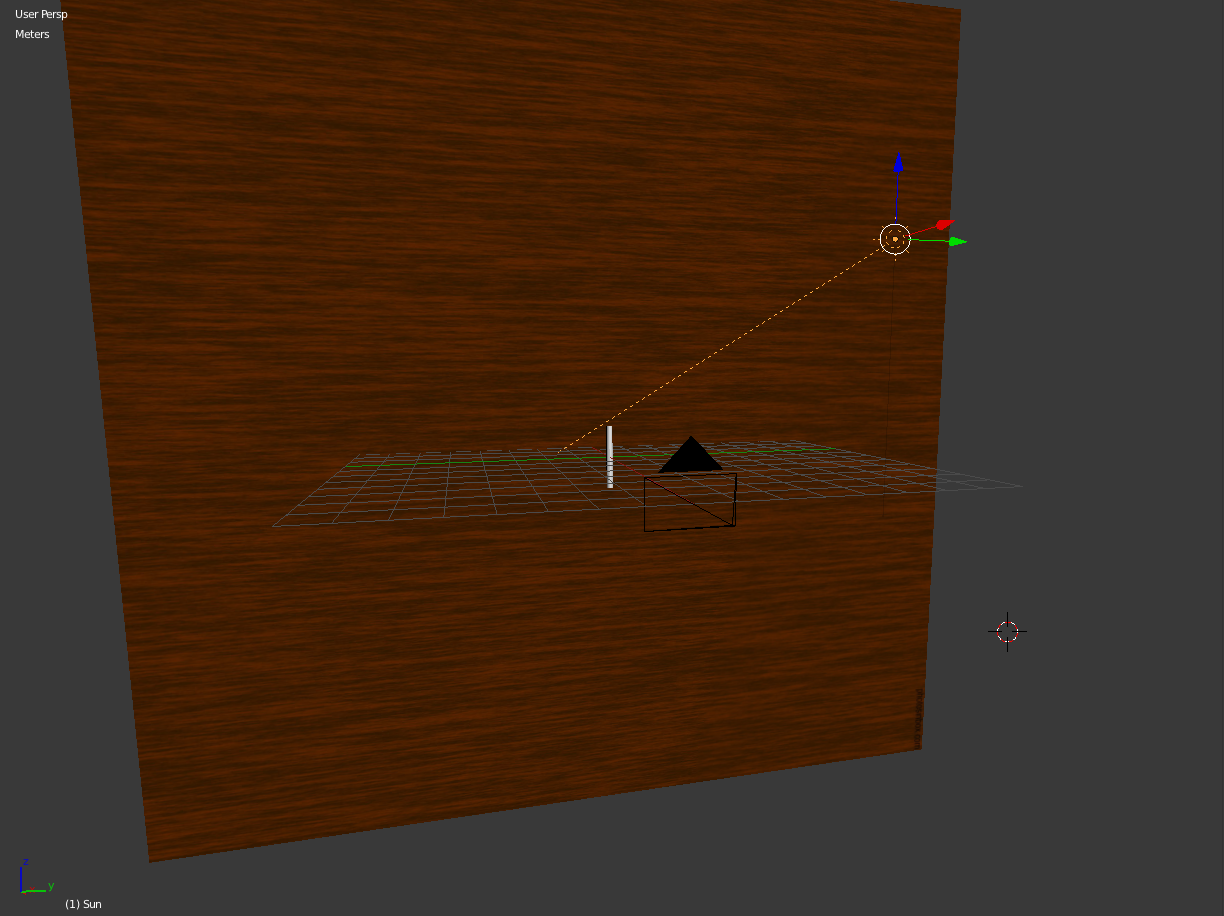
\includegraphics[width=0.5\textwidth]{./Template_Figures/blender_scene}
    \caption{Typical arrangement of the scene rendered with blender.\label{fig:blender_scene}}
\end{figure}

\subsection{Stereo and Automultiscopic stimuli}
For the stereo experiments, captured the scene with the camera baseline starting from 0.002 meters till 0.12 meters with the step of 0.002 meters. This gave us sixty sets of stereo images where the theoretical depth of the cylinder ranged from 0.13 cm to 3.45 cm in front of the plane of focus. Figure \ref{fig:stimuli_stereo} shows stereo images of one of the cylinder and the dragon. The step size was chosen small enough so that the transition from the minimum depth to the maximum for an object would seem continues to the observer.
\begin{figure}[htbp]
    % \centering
    \begin{subfigure}[b]{0.5\textwidth}
        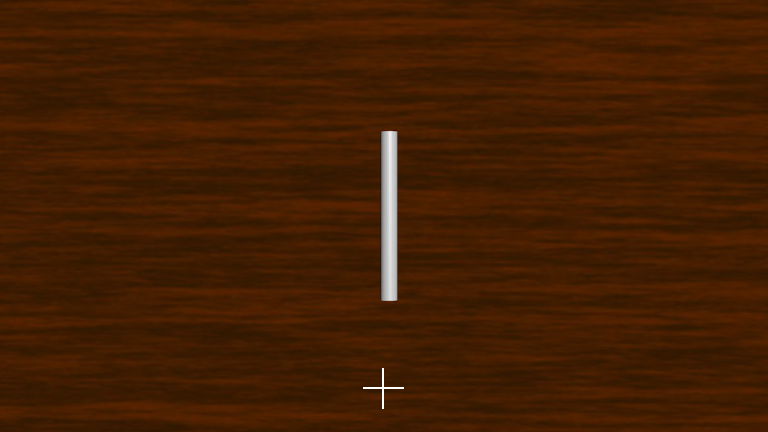
\includegraphics[width=\textwidth]{./Template_Figures/57L.png}
        \caption{}\label{fig:left_stereo_cyl}
    \end{subfigure}
    \begin{subfigure}[b]{0.5\textwidth}
        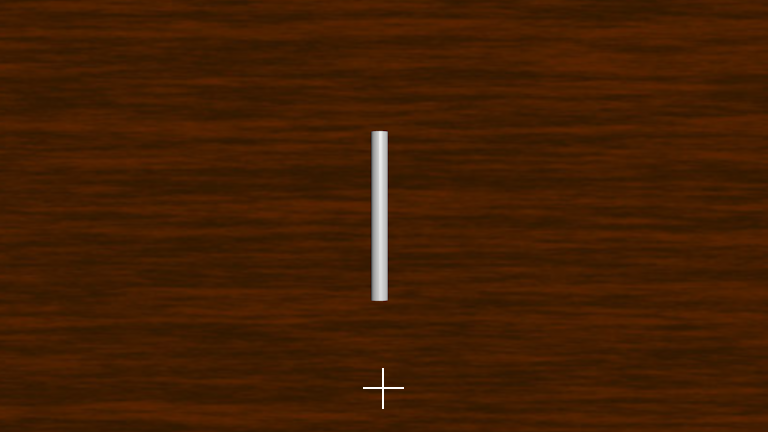
\includegraphics[width=\textwidth]{./Template_Figures/57R}
        \caption{}\label{fig:right_stereo_cyl}
    \end{subfigure}

    \begin{subfigure}[b]{0.5\textwidth}
        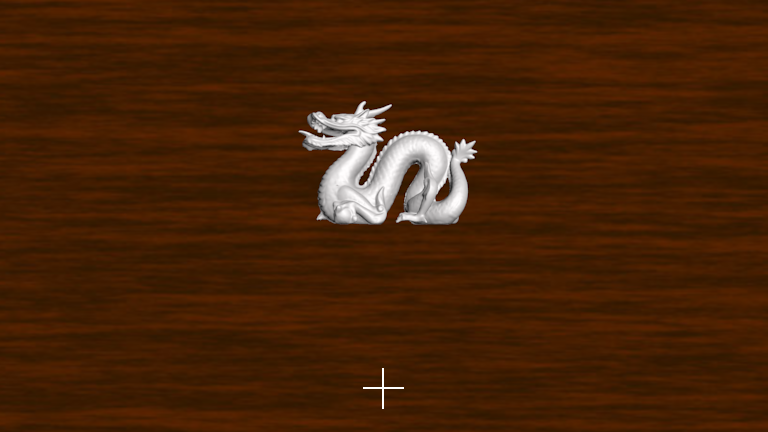
\includegraphics[width=\textwidth]{./Template_Figures/57Ld.png}
        \caption{}\label{fig:left_stereo_dra}
    \end{subfigure}
    \begin{subfigure}[b]{0.5\textwidth}
        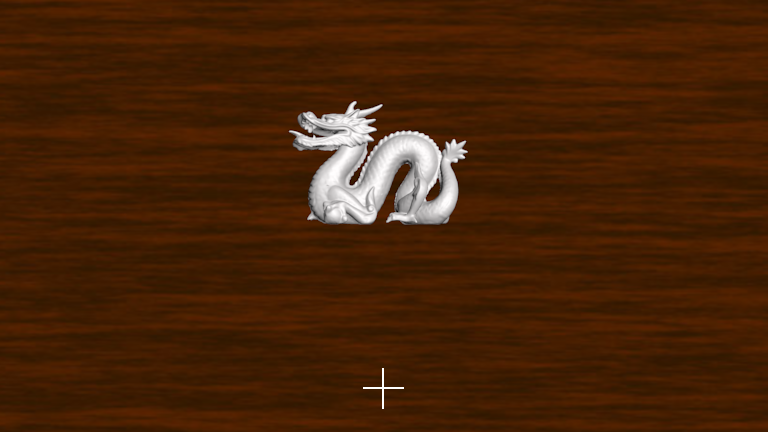
\includegraphics[width=\textwidth]{./Template_Figures/57Rd.png}
        \caption{}\label{fig:right_stereo_dra}
    \end{subfigure}
    \caption{Stereo images of the cylinder of 5 cm radius and the dragon. The theoretical depth difference between the objects and the backgroud is 3.44 cm. Viewer can cross-fuse to see in depth.\label{fig:stimuli_stereo}}
\end{figure}

The images for automultiscopic experiments were rendered similarly. The only difference being that the range of baseline started from 0 until 0.24 meters. The reason for this is explained in the next section.


\section{Apparatus and simulation procedure}

\section{subjects}

\section{Results}

\section {Discussion}
\subsection{Stereo}
\subsection{Automultiscopic}


% \subsection{Apparatus setup}
% \subsection{Experimentation Procedure}

% \subsection{Stereoscopic Experimentations}
% \subsubsection{Initial Hypothesis}
% \subsubsection{stimuli}
% \subsubsection{Simulation of Cross-talk}
% \subsubsection{Experimentation procedure}
% \subsubsection{Results}

% \subsection{Automultiscopic Experimentations}
% \subsubsection{Initial Hypothesis}
% \subsubsection{stimuli}
% \subsubsection{Simulation of Cross-talk}
% \subsubsection{Experimentation procedure}
% \subsubsection{Results}

% \subsection{Conclusion and Discussion}
% % read chapter "Matching corresponding images" from the oxford book "Binocular vision and stereopsis."

% % Section 2
% \section{HVS depth from disparity Model}
% \subsection{Different Hypothesis and their Outcome}
% \subsection{Future Work}


% % Section 3
% \section{Cross-talk Mitigation}
% \subsection{Proposed Optimizations}
% \subsection{Unsharp Masking in View Domain}
% \subsection{Iterative Subtraction}

